\chapter{Problem analysis}
We divide the analysis into three steps.
In the first section, we think of potential users of the integration in order to define realistic use cases for them.
Four use cases describe the user's intentions.
Then, we specify requirements, which are demanded by the use cases.
In the last section, we propose a high-level architecture of our solution, where we aim at utilizing Blazor and Peachpie to cover the requirements.

\section{Use Cases}
\change[inline]{Pojmenovat use casy}
We remind technologies of interest to introduce a context of our use cases.
PHP is used for server scripting, where it is designed to process a request, create the website, and send it back.
Blazor is a web framework for creating a client-side UI using C\#.
Peachpie is a PHP compiler, which compiles a collection of PHP scripts, representing a standalone project, to a .NET assembly.
\par
We consider four types of potential users.
The first type is a C\# programmer, Blake, excited to Blazor and read our thesis.
\par
The second type is a PHP programmer, Alice, who has no experience with Blazor but knows Peachpie basics.
Alice creates standard websites written in PHP, whereas she uses techniques introduces in the PHP section.
One day she wants to move the website to a client side.
Blake tells her about our thesis proposing a solution to migrate the scripts to a browser using Blazor and Peachpie.
She is excited by the solution and looks forward to using it.
However, she does not want to learn the Blazor framework.
Her point of interest is to use the solution for helping her to migrate her website to a browser.
The solution should provide an effortless manual on how to deploy it.
The manual should support most of the PHP conventions, which we could see in the PHP section.
\par
The third type is a PHP programmer, Bob, who has already tried to write a simple website using Blazor and knows Peachpie basics.
He creates standard websites similar to Alice's.
One day he wants to contribute to a website powered by Blazor.
He has a great idea of adding a new widget, which can be implemented by a few PHP scripts, which use some libraries.
Blake tells him about our thesis, and his wish is to use the solution to help him inject his scripts into the website.
The solution should be adopted to his skills.
\par
The fourth type is an enthusiastic PHP programmer, Chuck, who has advanced experience with Blazor and knows Peachpie basics.
He does not avoid exploring new technology to utilize all their aspects.
Again, there is an existing Blazor project, and he wants to add a new feature to it.
The PHP language offers the best way to implement it, but the feature is so render demanding that he wants to make use of Blazor to make the UI rendering more effective.
Blake tells him about our thesis, and Chuck wishes that the solution offers him to collaborate with Blazor by PHP.
\par
These descriptions should help us determine the following use cases, which are realistic to both potential users.
We call the first use case \textbf{Web} relating to Alice.
We suppose she has a simple PHP website, which contains some information about her company.
The website does not work with a database and consists of pages containing images and references interconnect them.
Some pages are adjustable by specifying the query part of the URL, and they include other scripts to add some basic layout.
One day the website notices many accesses, and Alice wants to migrate the website in order to a client side to save server resources.
The migration should download most of the website to a browser.
Afterward, navigation between scripts and script execution should be maintained on the client side.
Even more, Alice does not want to adjust the website for a client side too much, and she wishes for a simple solution that is understandable by a novice.
\par
We call the second use case \textbf{OneScript} aiming at Bob, who already has some experience with Blazor.
There is an existing Blazor website, and he has an idea of a brilliant widget displaying the user's graph by HTML.
Because he is used to PHP, the HTML is rendered by PHP scripts.
The idea consists of let the user choose to load graph data from a file or generate a predefined graph as a demo.
After that, the widget renders HTML markup representing the graph.
Bob uses forms to interact with a user.
Unfortunately, Bob uses forms to interact with a user, and he is not willing to learn Javascript or interoperability between PHP and Blazor.
Thus, he needs a solution, which offers interaction with a user and uses standard PHP conventions mentioned earlier.
\par
We call the third use case \textbf{PhpComponent} relating to Chuck.
He wants to create a real-time web game similar to Asteroids written in PHP.
PHP programmers have not been used to saving variables or defined functions across scripts because of the HTTP policy mentioned in the PHP section.
Now, Chuck wants to try a new approach, where he relies on state persistent and saves a state of all game entities in variables.
One script execution should render one game scene as an HTML markup.
There is a timer, which executes the scripts every defined period of time.
The game is render demanding due to redrawing the scenes.
So he decides to target on a client side and utilizes Blazor, Peachpie, and our solution.
A client side execution should prevent network latency by loading the game in the beginning.
After that, the game will be independent of the network connection due to running the game and saving the game state by a browser. 
Because he has previous experience with Blazor infrastructure, he will appreciate utilizing all Blazor aspects to run this game.
Thus, he needs some representation of Blazor in PHP, which he will use for interacting with a browser.
\par
\begin{figure}[t]\centering
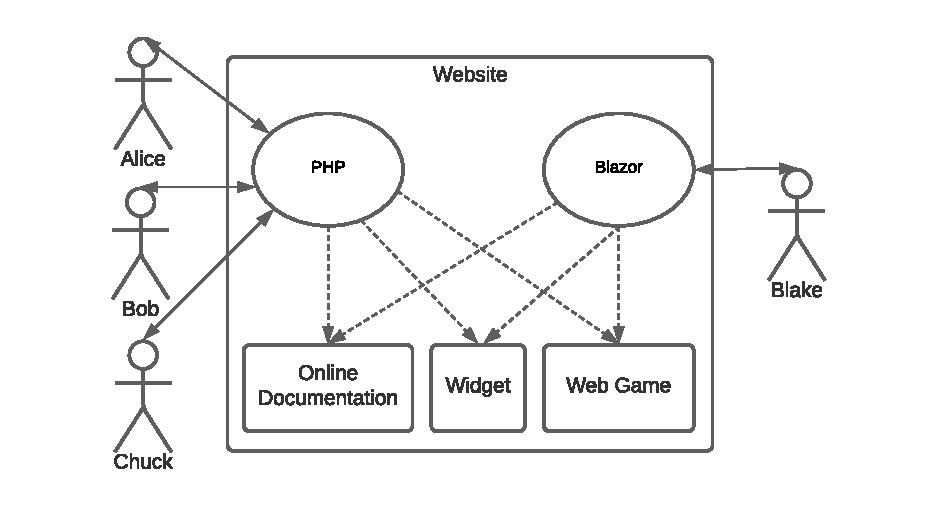
\includegraphics[scale=0.8]{./img/UseCaseAllTogether}
\caption{The AllTogether use case describing the combination of the rest. Double-headed arrows represent the person's used language. Dashed arrows represent a possible usage, where the head aims to an implementation written in the language.}
\label{img09:usecase}
\end{figure} 
\par
We can see an illustration of the fourth use case, which we call \textbf{AllTogether}, in Figure \ref{img09:usecase}.
The goal of the use case is to allow collaboration between PHP and Blazor programmers, where a difference of languages is not a barrier.  
We can image two teams creating a web application. 
They agreed on developing a client-side web application, where both teams aim at different parts of the website.
For example, one team wants to create a fun zone where a user can play some web game, we can imagine something like Asteroids, and the second team wants to create some online documentation about the game and the widget for the graph representation mentioned in \textit{OneScript}.
Because Blazor targets client-side web applications, they want to utilize Blazor.
Unfortunately, these teams use a different favorite language, where the first team uses PHP and the second team uses C\#.
Even more, these teams want to arbitrarily choose what part they want to develop.
They need some environment where the PHP team can code alongside the Blazor team, and they can focus on an arbitrary part of the web application.
We can see the intention in Figure \ref{img09:usecase} where each team can create a part aiming at the web game, the online documentation, and widget.
We can see the PHP team consists of Alice, Bob, and Chuck, having different skills with Blazor, so the environment should reflect it.
Even more, Blake should be able to manipulate their part of the application to customize it using C\#. For example, he should change the layout of the website without complex refactoring. 

\section{Requirements}

We will define requirements based on mentioned use cases.
\change[inline]{Cilem teto sekce je popsat pozadavky ktere kdyz budou naplnene tak..}
The question is what things should be enabled by the solution to make PHP scripts a valuable part of a Blazor website.
\par
\textbf{Navigation} is the first requirement that our solution should maintain.
We demonstrate navigation posibilities in the figure \ref{img10:scripts}.
Basic functionality should provide script routing, which finds a script by its name and executes it.
The solution should offer a straightforward router making a Php website accessible, as we can see in the figure.
A script should be injectable to a standard Blazor component due to the use case two, where the programmer injects a feature, written in PHP, to a Blazor page.
The simplicity is a necessary condition for programmer A and should be reflected.
The last option is a Blazor component in \texttt{script.php} enabling to use of already created components in PHP code.
\par
\change[inline]{Popsat ten obrazek a otocit jak to popisuju a nechat tam jen Vyhodit Blazor compnent ve script.php}
\begin{figure}[!b]\centering
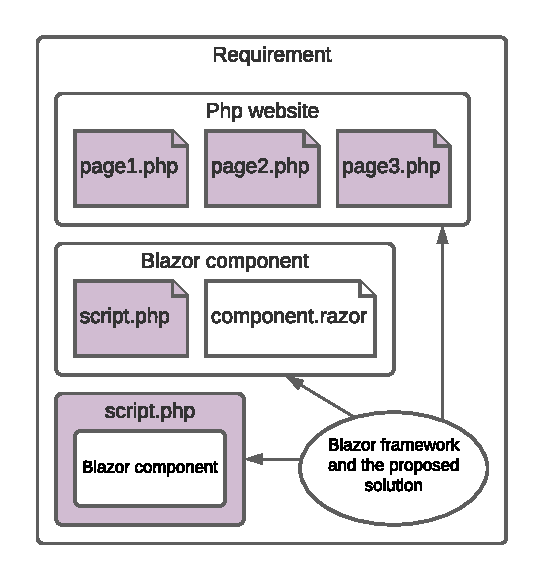
\includegraphics{./img/Requirement}
\caption{Scripts should be flexible.}
\label{img10:scripts}
\end{figure} 
\par
\textbf{Rendering} should be maintained in two ways.
The first way aims at programmer A when a script output is transparently displayed as a web page or its fragment.
The approach hides Blazor infrastructure for rendering a markup and makes creating a UI easier for PHP programmers.
The second way aims at programmer B when the solution provides an interface for the interaction with Blazor.
It is also necessary when we want to use already defined components in a PHP code.
\par
\change[inline]{Popsat co je ten state}
\change[inline]{Rozepsat jsou zvykli zanik requestu po kazdym requestu ale pro interakci s uzivatelem ji potrebujou zachovavat}
\textbf{State preservation} is a new feature, which should be available for creating a web application saving its state.
The example we can see in the use case 3 when we have to save the game state.
However, we should be able to choose whether it is intended behavior because scripts lose their state after every request on a server side.
\par
\change[inline]{Server simulation}
\textbf{Server abstraction} should be the main advantage of the solution.
We could see superglobals are commonly used methods how to obtain information about navigation or submitted data.
The solution should supports superglobals for examples like the use case 1, where the website uses information about URL query part, via \texttt{\$\_GET} variable, to make decisions.
\par
\textbf{Forms} should be maintained by the solution. 
They should not be sent to a server but parsed and provided in superglobals. 
After navigation to a script defined in the \texttt{action} attribute, the script should access the form data.
\change[inline]{relates ne tyka se }
Data processing also relates to files, when it should be possible to upload and download files.
\par
\textbf{Interoperability} between PHP and Javascript should be supported for situations when forms, the server abstraction, or Blazor are not sufficient.
We should be able to call Javascript functions from PHP and vice-versa.

\section{Architecture}

\change[inline]{Colekce scriptu}
The basic principle of our solution consists of a PHP script compilation into .NET assembly by Peachpie.
After that, a Blazor App references the assembly with a support library, providing a mechanism for navigating and executing the scripts.
\change[inline]{Zminit rovnou jeji jmeno v predchozi vete}
From now on, we will call the library \texttt{Peachpie.Blazor}.
Then, a server serves the application to a browser, where Mono runtime executes it.
We will describe the architecture from the view point of compilation time and runtime.
\par
When we think about PHP script compilation, there are two possibilities.
We can compile the scripts ahead of time and reference them from a Blazor App, as we can see in figure \ref{img11:compilation}. 
The second way is to regard the scripts as Static Web Assets and load them into a browser as scripts.
Afterward, the Peachpie compiles and executes them.
Both approaches have different advantages. 
Thus, there is no silver bullet.
The first approach saves time by ahead compilation and compilation check.
However, the second approach can save browser memory when the web application is larger, and a client uses only a part of it.
Since we have to choose, we are inclined to the first approach.
\change[inline]{Je to stabdartni zpusob jak se to v peachpie dela}
\par
\change[inline]{Dat to pric}
\begin{figure}[!b]\centering
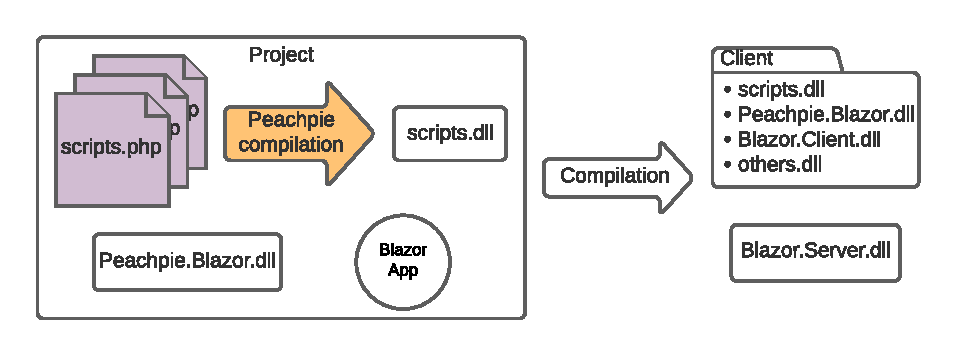
\includegraphics[scale=0.8]{./img/Compilation}
\caption{Compilation.}
\label{img11:compilation}
\end{figure} 
\par
We have to figure out how to attach a PHP code, which is compiled into the assembly, to the Blazor App.
\change[inline]{Peachpie to deafaultne podporuje}
Although, we can now call functions written in PHP from Blazor, we want to create an abstraction over the Blazor environment in order to simplify the interface.
The abstraction should offer a representation of PHP scripts in Blazor.
It should allow an option for accessing the Blazor interface for advanced features.
It should be compatible with the Blazor environment in other to allowing a smooth collaboration between the abstraction and the Blazor pages.
A Blazor page consists of components.
We can achieve collaboration by utilizing the component to represent PHP scripts.\change[inline]{Odstranit nasledujici}
We can benefit from a component architecture.
Componets can be arbitrarily put together, which offers to place our PHP section in the desired place in the Razor code.
\change[inline]{Priblizit}
Even more, we can replace \texttt{Router} with the component representing PHP scripts.
Afterward, scripts will care about the whole Blazor website content.
The component provides a sufficient Blazor interface for rendering control and interaction with a browser. 
We can illustrate the options of usage in figure \ref{img12:component}.
\change[inline]{Odkaz an nej drive}
\par
\begin{figure}[t]\centering
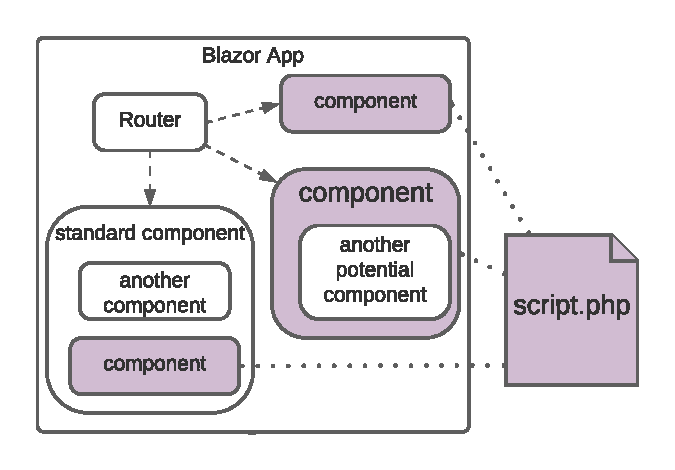
\includegraphics{./img/component}
\caption{The component representing a PHP script.}
\label{img12:component}
\end{figure} 
\change[inline]{Uprasnit v obrazku vice scriptu}
\change[inline]{dovysvetlit sipky}
\par
We can think about how to represent PHP scripts as components.
There can be one type of component, which will provide the abstraction for all the PHP code in scenarios.
A problem with this approach is that the use cases need different levels of abstraction.
The third use case wants to use the component for offering the Blazor interface accessible from PHP code.
The offer should contain identical or similar options, which are given in a C\# code.
The second use case wants to use the component as an adjustable provider.
The provider finds and executes PHP scripts.
Its purpose is to keep the user away from knowing about the detailed structure of Blazor and the integration.
Another important thing is a provider role in a Blazor App.
The provider can behave either as the Router or as a navigatable component, which enables the navigation of PHP scripts.
\change[inline]{As a result...for different proposes}
The conflict yields to create more types of components.
These types will provide the abstraction for the particular scenarios.
The solution will reach two types of components.
The first one wants to bring Blazor to PHP in order to utilize the whole environment.
The second one aims at presenting a transparent execution of standard PHP script without strangeness of connection between Blazor and PHP.
\change[inline]{Jinak zformulovat, bez toho aby se o to musel zajimat}
\par
We will focus on the first component.
We will call the component \texttt{PhpComponent} due to the effort of moving the component concept to PHP.
\texttt{PhpComponent} aims at the third use case.
Despite language's differences, we can utilize the common concept of classes and inheritance.
Peachpie allows inheriting C\# class in a PHP code.
This feature results in full support of component interface without creating new structures for managing component's behavior from PHP.
We can inherit \texttt{ComponentBase} class in PHP and use its methods in the same way as C\# class.
The inheritance offers the required interface for creating effective rendering in scenario 3.
There are also subproblems with the differences.
The current Peachpie version does not support some C\# specifics fully.
The reason can be a hard or impossible representation of C\# entities in PHP.
It should be developed some PHP support for making the usage of the interface easier.
The support will replace the missing usage of the interface.
\par
We will call the second type of component \texttt{PhpScriptProvider} expressing an environment for executing standard PHP scripts.
\texttt{PhpScriptProvider} aggregates the requirements of the rest scenarios by a single component.
Although, the provider has more than one purpose.
The main idea of serving a PHP code is the same.
The provider should be able to navigate and execute PHP scripts.
Because the rest scenarios try to hide the integration, the provider should support the following features.
It should pretend a server behavior.
The behavior contains rendering everything, which is outside the PHP section or written by echo.
Superglobals are often used for obtaining additional information given by the user.
An ability to fill \texttt{\$\_GET} variable with the URL query part should be presented.
It should change a standard form functionality to saving the form information into superglobals and execute the script again.
Loading and saving files submitted by form is essential for avoiding using Javascript.
There is an interesting thing about saving the script context to the next execution.
These abilities are the same for the rest scenarios.
We will describe the provider modes.
These modes are intended to solve the rest use cases. 
\par
The first mode relates to the first use case.
It enables to set the provider as a root component.
It handles all navigation events, determines the script name, finds it, and executes the script.
PhpComponents can also be a navigation's target.
\par
The second mode relates to the second use case.
It enables the provider insertion into a Razor page.
Afterward, the provider executes the specified script.
\par
The third mode relates to the last use case.
It enables to navigate the set of scripts with respect to URL.
The navigation is generally maintained by the default \texttt{Router}.
The component only provides navigation to scripts.
\par
We can see that two different components are rational ways how to separate the problems and offer an understandable difference between the components.


